\section{Begrifflichkeiten}
\begin{frame}
	\frametitle{Pr"ufsummen}
	z.B. eine Quersumme "ueber eine Zahl.

\end{frame}

\begin{frame}
	\frametitle{Problem}
	Zu einer gegebenen Pr"ufsumme kann jeder\\
	eine valide andere Zahl generieren.
\end{frame}

\begin{frame}
	\frametitle{Hashfunktionen}
	\begin{center}
		Hashfunktionen sind Einweg-Funktionen\\
		die eine beliebig grosse Datenmenge\\
		auf eine kleinere Datenmenge abbilden.\\
		\vspace{1cm}
		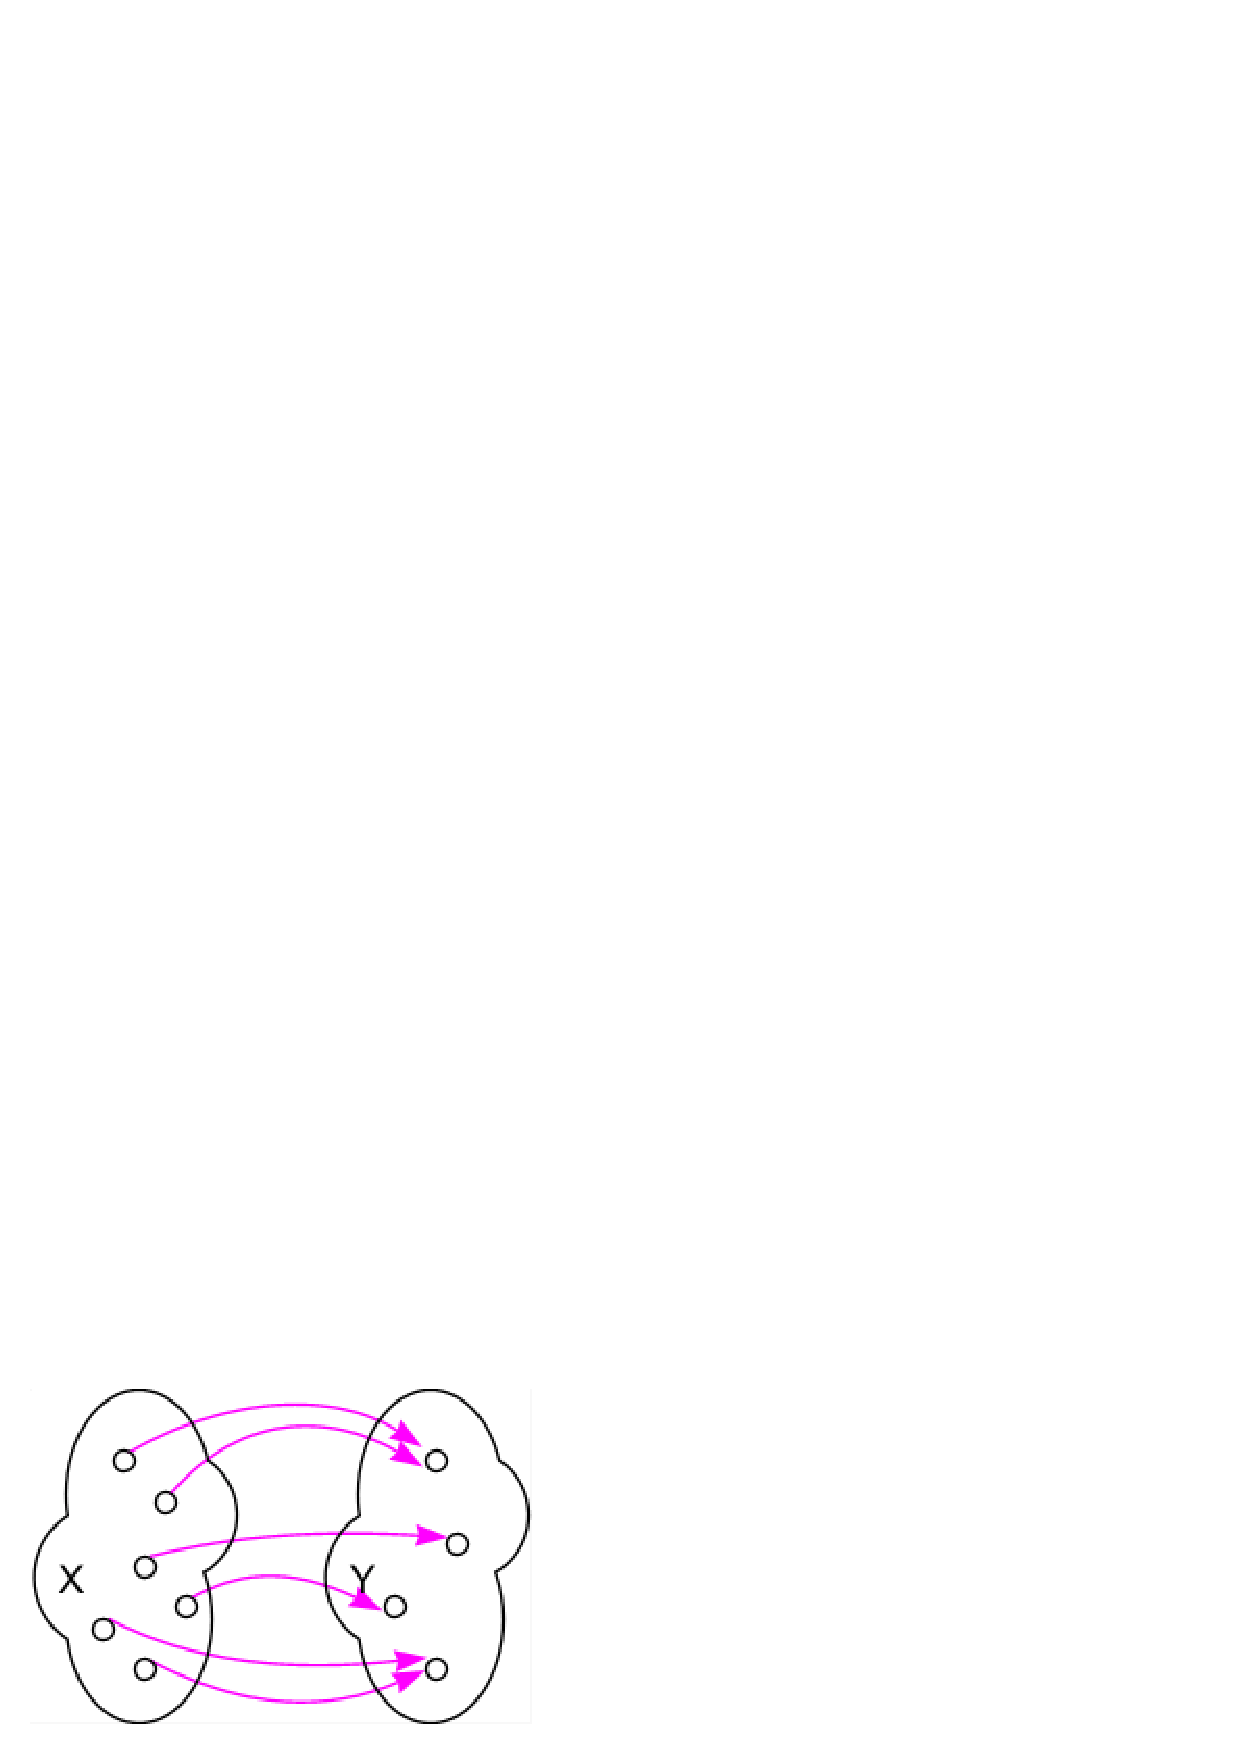
\includegraphics[width=4cm]{surjektiv.png}
	\end{center}
\end{frame}

\begin{frame}
	\frametitle{Hash-MACs}
	\begin{center}
		Hash-MACs sind Hash-funktionen zur\\
		Authenfikation von Nachrichten.
		\\
		\begin{center}
			$HMAC_k(msg) = hash((k \oplus opad) \parallel hash((k \oplus ipad)\parallel msg) )$
		\end{center}
	\end{center}
\end{frame}
